\documentclass[border=5pt]{standalone}
\usepackage{tikz}
\usetikzlibrary{calc, positioning}
\usepackage{amsmath}
\begin{document}
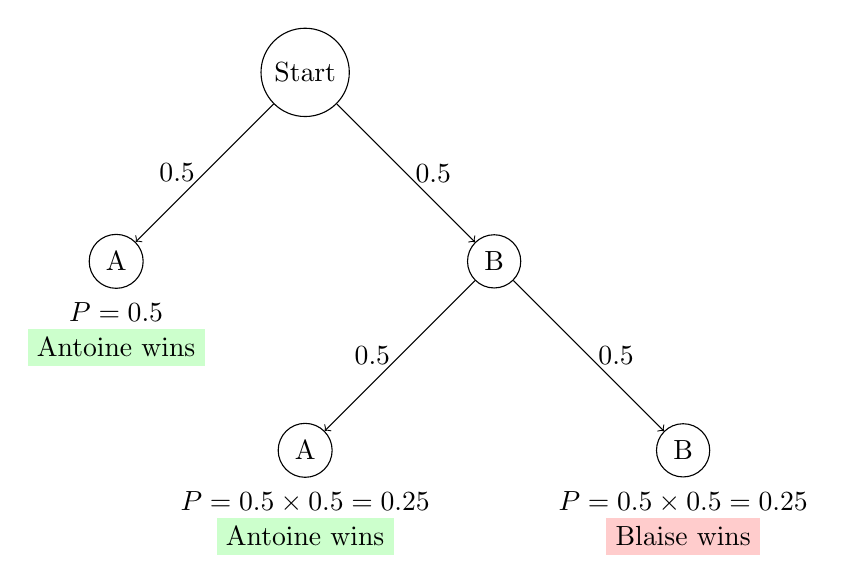
\begin{tikzpicture}[scale=1.2]
% Tree diagram
\node[draw, circle] (start) at (0,0) {Start};
\node[draw, circle] (A1) at (-2,-2) {A};
\node[draw, circle] (B1) at (2,-2) {B};
\node[draw, circle] (A2) at (0,-4) {A};
\node[draw, circle] (B2) at (4,-4) {B};

% Edges with probabilities
\draw[->] (start) -- (A1) node[midway, left] {0.5};
\draw[->] (start) -- (B1) node[midway, right] {0.5};
\draw[->] (B1) -- (A2) node[midway, left] {0.5};
\draw[->] (B1) -- (B2) node[midway, right] {0.5};

% Game outcomes
\node[below=0.5cm of A1, fill=green!20] {Antoine wins};
\node[below=0.5cm of A2, fill=green!20] {Antoine wins};
\node[below=0.5cm of B2, fill=red!20] {Blaise wins};

% Path probabilities
\node[below=0.05cm of A1] {$P = 0.5$};
\node[below=0.05cm of A2] {$P = 0.5 \times 0.5 = 0.25$};
\node[below=0.05cm of B2] {$P = 0.5 \times 0.5 = 0.25$};
\end{tikzpicture}
\end{document}
